%%%%%%%%%%%%%%%%%%%%%%%%%%%%%%%% 
\section{The Light-Readout System} 
\label{sec:detectors-fd-alt-light}

The light-readout system developed in the LAGUNA-LBNO design study
detects the scintillation light using 8-inch cryogenic
photomultipliers (Hamamatsu R5912-02mod) with TPB coating. The PMTs
are placed about 1~m below the cathode.  The application of the TPB
coating can be done at the level of the glass itself or on a
transparent plate mounted over the photocathode surface. The WA105
demonstrator will use 36 photomultipliers R5912-02mod (1/m$^2$ of
cathode surface). The mechanics for the PMTs' attachment has been
carefully studied; it must counteract the PMT buoyancy while avoiding
stress to the PMT glass (due to differentials in the thermal
contraction between the support and the PMT itself).

The dual-phase LAr detectors designed for LBNO are equipped with a
large number of PMTs. Depending on the size of the detector and on the
density of PMT on the detection surface, this number may be as high as
1000. The large number of photosensors called for a large integration
scale solution for the front-end electronics.

Solutions of this kind have been studied, in the framework qof the
R\&D program PMm2 \cite{PMM2-1, PMM2-2}, for the instrumentation of
giant water Cherenkov detectors with photomultipliers. The signal
digitization is performed by grouping the photomultipliers in arrays
of 16. Each photomultiplier array is read out by an ASIC chip in AMS
SiGe 0.35~$\mu$m technology. The ASIC, which is called PARISROC
(Photomultiplier ARrray Integrated in Si-Ge Read Out
Chip)\cite{Parisroc}, provides a complete readout system for
triggerless data acquisition. The solution developed by this program
represents an important handle for cost reduction.


%\begin{cdrfigure}[Layout of the PARISROC ASIC]{parisroc}{Layout of the PARISROC ASIC used for the production of the second iteration of the chip (from Nucl.Instrum.Meth. A623 (2010) 492-494).}
% 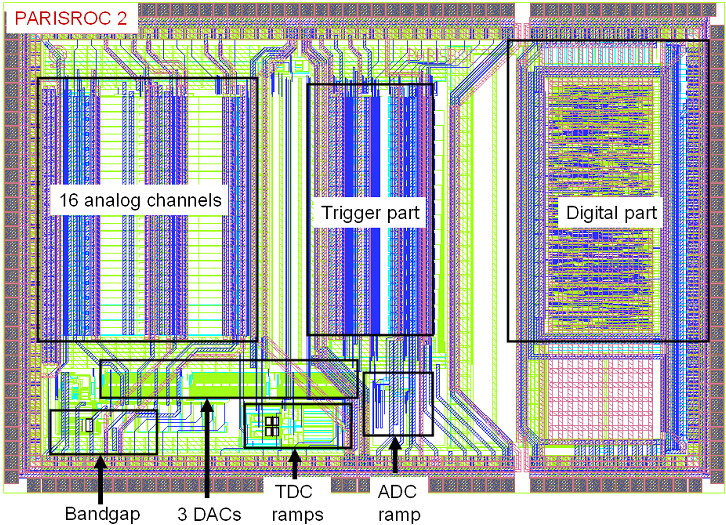
\includegraphics[width=.5\textwidth]{PARISROC2}  
%\end{cdrfigure}

The front-end electronics for the light readout of the WA105
demonstrator will be based on the solution developed by the PMm2
R\&D. The PARISROC ASIC, as described in the following, is currently
adapted to the time structure of the scintillation light produced in
the interactions of secondary particles in neutrino interactions in
LAr. The detection of the direct scintillation light (S1) that
provides the absolute event time is the main task of the electronics.
The electronics will also process the signals from the scintillation
light (S2) produced by the electrons as they are extracted and
amplified in the gaseous phase.


The PARISROC chip reads the signals of 16 photomultipliers
independently of one another. Each analog channel consists of a
low-noise preamplifier with variable and adjustable gain (8 bits) to
compensate for the relative photomultiplier gain differences when
powered by a single high voltage. The preamplifier is followed by a
slow channel for the charge measurement in parallel with a fast
channel for the trigger output. The slow channel includes a variable
(50--200~ns) slow shaper followed by an analog memory with depth of 2
to provide a linear charge measurement up to 50~pC; this charge is
then converted by a 10-bit Wilkinson ADC. The fast channel is composed
of a fast shaper (15~ns) followed by a low offset discriminator to
auto-trigger down to 10~fC. This auto-trigger feature makes the PMT
array completely independent of from the other PMT arrays. The
threshold is loaded by an internal 10-bit DAC common to the 16
channels.

%\begin{cdrfigure}[Block diagram of the PARISROC ASIC.]{block-diag}{Block diagram of the PARISROC ASIC.}
 %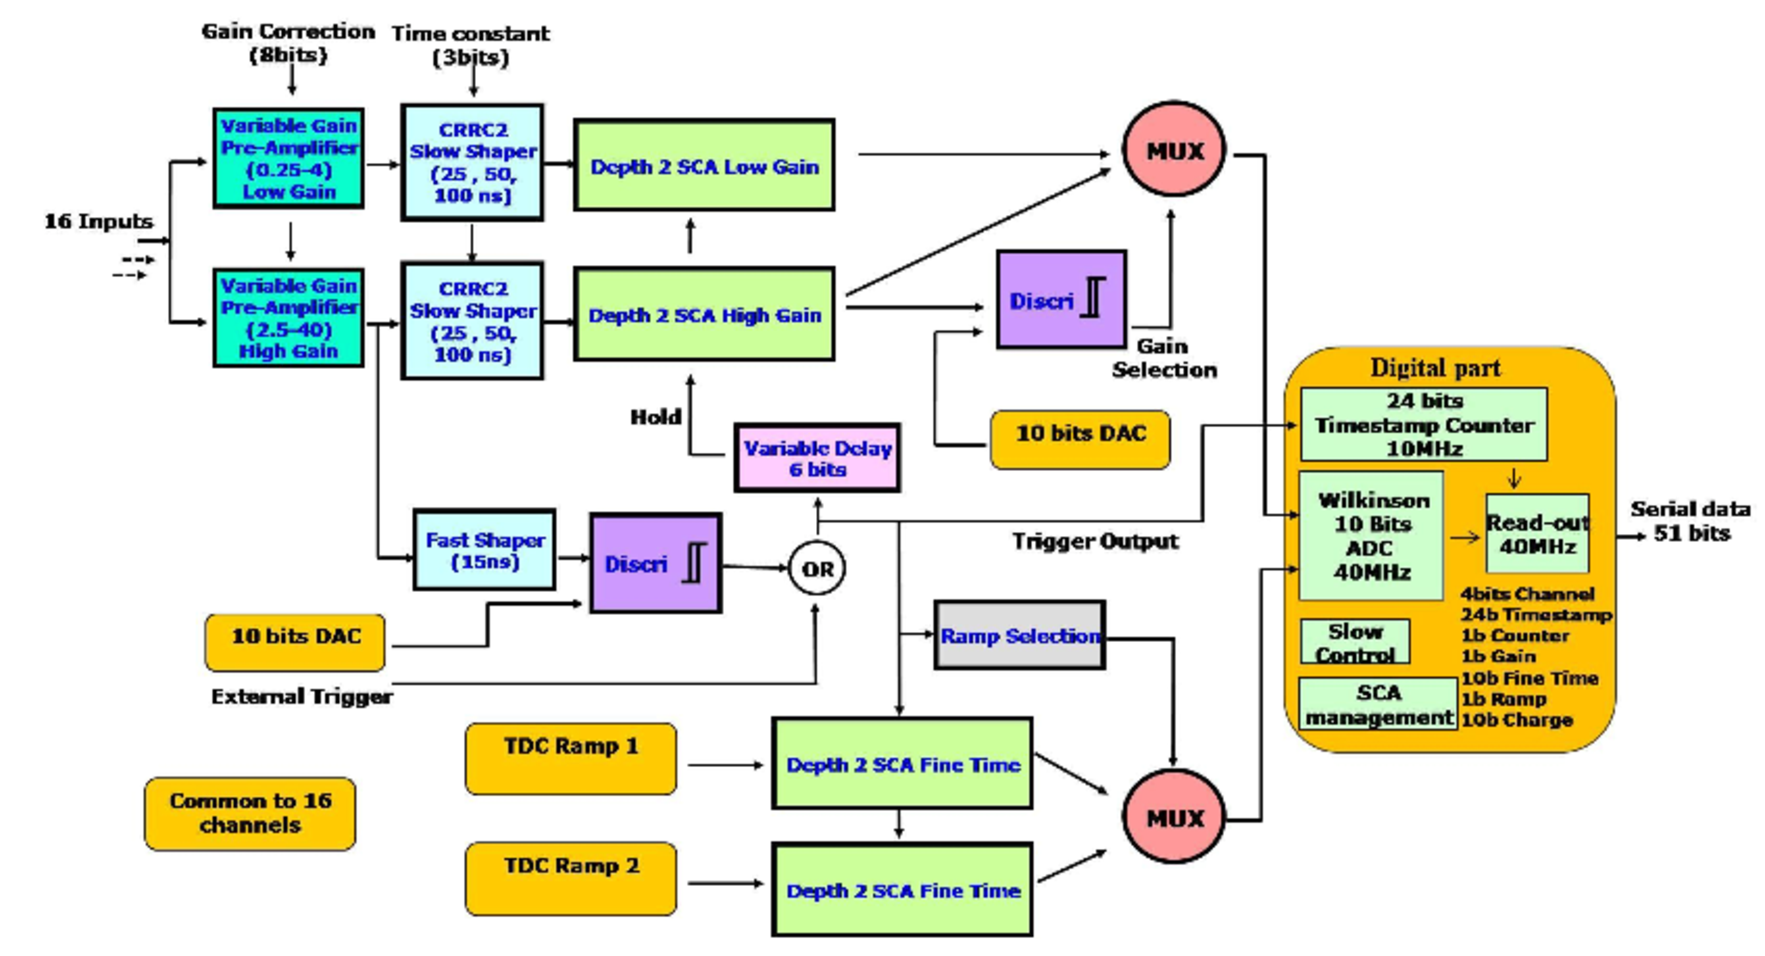
\includegraphics[width=.7\textwidth]{parisroc_blockdiag.pdf}  
%\end{cdrfigure}

The variable gain of each preamplifier provides the flexibility to
adapt the system to the characteristics of each photomultiplier after
it has been correctly calibrated. In the timestamping process, there
are two TDC ramps working in phase opposition in order to reduce the
dead time (when the ramp goes to zero) by selecting the other ramp,
that will be in its active state.

When an event occurs, the value of the correct ramp is digitized and
inserted into the data stream that includes: a 24 bit counter that
goes much more slowly than the ramps in order to have a coarse time
measurement, a flag that indicates which ramp has been digitized, an
ID of the channel triggered, and the timestamp and charge information.

%\begin{cdrfigure}[MicroTCA rack and Bittware S4AM board]{LRO-rack}{MicroTCA rack and Bittware S4AM board}
 %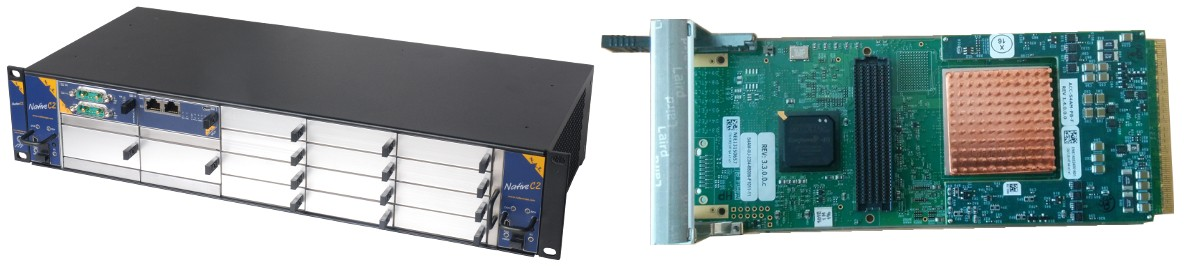
\includegraphics[width=.6\textwidth]{rack}  
%\end{cdrfigure}

The light readout is fully integrated in the WA105 DAQ scheme. A
microTCA crate housing the light-readout digitization cards is
naturally integrated into this architecture by taking into account the
common time distribution and data transmission systems.  During the
data-taking outside the beam spills, a trigger that can be generated
by the light-readout microTCA crate plus its timestamp can be
transmitted over the White Rabbit network similarly to the beam
triggers.

On the light-readout front-end board there is also an ADC (AD9249 from
Analog Devices) that digitizes the PMT charge information on every
channel independently. The charge measurement can be correlated with
the timing information coming from the PARISROC for better precision
on both quantities. A prototype of the light-readout AMC is also being
developed by using the Bittware development card S4AM (the same used
for the LAr TPC ionization readout developments) and a mezzanine card
including the ADC and the trigger circuit (see
Figure~\ref{fig:DAQ_LRO}).
\begin{cdrfigure}[Block diagram of the light readout AMC demonstrator card]{DAQ_LRO}{Block diagram of the light readout AMC demonstrator card}
 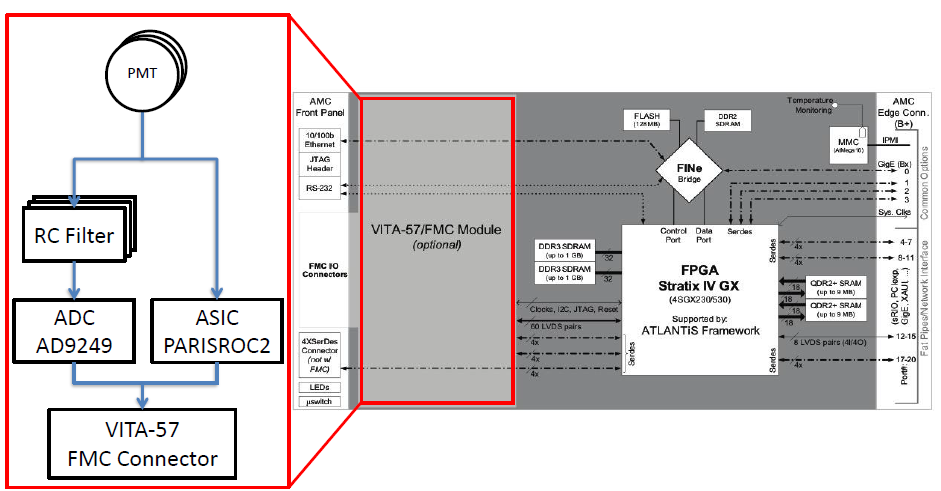
\includegraphics[width=.6\textwidth]{DAQ_LRO}  
\end{cdrfigure}

The PARISROC chip provides the timestamp at nanosecond precision and
generates the trigger. In parallel, an ADC AD9249 continuously
digitizes all channels independently at 65~MSPS with 14 bits. The FPGA
Stratix IV from the Bittware S4AM card controls and programs the ADC
and PARISROC. It also receives the data coming from both PARISROC and
ADC and controls which information is passed through the network to
store for analysis.  The charge digitization of the light signals is
performed at 14~bits in samples of 15~ns. Considering a 5~$\mu$s
light-signal duration, the digitization will produce more than 300
samples. With this amount of data it is possible to measure not only
the total charge generated but also the shape of the signal and the
long-component decay of the light.

%The firmware of the FPGA is in its early stage of development and there is still an open debate about which information will be useful. It will definitively include the time stamp of every event on each channel as well as the digitization of the charge received in each of them. Some questions concern the duration of the PMT sampling and the feasibility of including some real-time processing. This could include an inverse filter of the RC circuit to compensate its contribution.

With this light readout architecture and the White Rabbit
time-distribution system, it is possible to achieve 1-ns accuracy at
the level of trigger generation for the T0 and timestamping of the
events. This trigger is sent to the general DAQ and the event
builder. Since the charge-readout system of the TPC runs at 2.5~MHz,
the minimal time unit in the reconstruction of the drift is 400~ns.
